\begin{savequote}[6cm]
<< If you will remember back,\\ The words I spoke were quite exact. >>
\qauthor{Zecora}
\end{savequote}

\chapter{Expressivité d'Astral}\label{chap:validation:expressivite}
\chaptertoc

Dans le chapitre~\ref{chap:contrib:astral}, nous avons présenté Astral, une algèbre pour exprimer des requêtes continues sur flux et relations. Nous avons jusqu'ici présenté principalement des définitions, mais nous n'avons pas encore listé de propriétés formelles. Or, ces propriétés ont des impacts forts dans le cadre de l'optimisation de requêtes.

Ce chapitre permet d'analyser plus en profondeur cette algèbre et d'en explorer ses capacités et limitations. Afin de valider nos choix, nous analysons la puissance d'expression résultante ainsi que les capacités de démonstration de propriétés que nous obtenons.

En premier lieu, nous détaillons en section~\ref{sec:valid:expressivite:modele} les choix concernant les définitions fondamentales en les comparant avec l'état de l'art. Par la suite, dans la section~\ref{sec:valid:expressivite:comparaison}, nous comparons l'expressivité d'Astral avec les autres modèles théoriques de la littérature. Dans la section~\ref{sec:valid:expressivite:theoremes}, nous explorons les capacités de cette algèbre en démontrant des théorèmes non triviaux d'équivalence de requêtes et de transpositions. Puis, nous concluons par une synthèse dans la section~\ref{sec:valid:expressivite:conclusion}.
\section{Choix des fondations de l'algèbre}
\subsection{Continuité du temps}
\subsection{Sémantiques d'ordres}
\subsection{Hypothèse de la cohérence temporelle}
\subsection{Équivalence de requêtes}
\section{Comparaison de l'expressivité d'Astral}\label{sec:valid:expressivite:comparaison}
L'algèbre Astral a été conçue pour permettre d'exprimer des requêtes continues sans ambiguïté, mais aussi pour introduire de nouveaux opérateurs afin d'étendre la puissance d'expression des requêtes continues. Dans cette section, nous analysons en détail son expressivité. En premier lieu, nous détaillons qu'Astral couvre naturellement un large ensemble des approches actuelles. Ensuite, nous analysons les opérateurs que nous avons particulièrement remodelés : les séquences de fenêtres et la manipulation temporelle.

\subsection{Expressivité générale}
Astral est inspiré de l'algèbre \textit{ACO} de \textit{STREAM}. Nous avons repris la majeure partie des idées, notamment celle d'avoir des flux et des relations, et avons appliqués nos définitions plus strictes, comme nous l'avons vu dans la section précédente. Nous pouvons affirmer que nous couvrons l'expressivité de \textit{STREAM}.

Sachant que \textit{STREAM} a démontré dans~\cite{Arasu:stream} que son expressivité couvre les approches de l'époque comme \textit{Chronicles}, \textit{Tribeca}, \textit{NiagaraCQ} ou \textit{Aurora}. Nous pouvons considérer qu'Astral est, par transitivité, plus expressive que ces travaux.

Notre formalisation à base de \textit{batch} nous permet de supporter les sémantiques exposées par~\cite{Jain:spread}. Nous avons de même présenté notre interprétation des opérateurs \textit{SPREAD} correspondant aux définitions décrites. Il est toutefois notable que les parties où les auteurs spécifiaient des choix non-déterministes ont été remplacés par des choix sur l'ordre positionnel.

Nous avons vu que Astral couvrait une grande partie des approches actuelles. Nous allons maintenant nous concentrer sur l'opérateur le plus étudié de la littérature : les séquences de fenêtres.

\subsection{Fenêtres}
Dans cette section, nous analysons l'expressivité des séquences de fenêtres. Afin de voir les capacités de notre formalisation, nous revisitons les expressions de fenêtres présentés dans l'état de l'art. Nous commençons par la sémantique la plus largement utilisé de la fenêtre glissante \textit{RANGE}/\textit{SLIDE}.
\subsubsection{RANGE $x$ SLIDE $y$}
Dans le cadre de la fenêtre glissantes, il existe deux descriptions possibles. La définition exacte telle que présente dans plusieurs travaux et telle que spécifiée dans~\cite{Jain:spread} est la suivante :

\DSF{r = y}{\beta(j) = yj+t_0}{\alpha(j) = \max(yj-x,0)+t_0}

Comme spécifié, les premiers états des bornes ont une largeur de fenêtre plus petite que $x$. Dès que $j \geq \frac xy$, alors la largeur temporelle deviendra égale à $x$. Nous pouvons noter que la fonction $\alpha(j) = yj-x+t_0$ n'est pas valide dans notre contexte. La seconde condition des DSF (def~\ref{def:dsf}) nécessite $\alpha \geq t_0$, ce qui n'est pas vraie pour $i=0$. L'insertion de la fonction $\max$ rend la description viable et décrit la sémantique des premières phases, ce qui n'est pas explicite dans sa description textuelle.

La description suivante est aussi valide, mais ne possède pas de phase initiale. Ici, la relation temporelle est vide jusque $\beta(0)$ afin d'assurer que la fenêtre couvre toujours une largeur temporelle de $x$.

\DSF{r = y}
	{\beta(j) = yj+x+t_0}
	{\alpha(j) = yj+t_0}

Afin d'illustrer les différences entre les deux sémantiques possibles, la figure~\ref{fig:valid:expressivite:slidemax} représente les différences d'évaluations pour une fenêtre glissante avec $y=2$ et $x=4$. Dans le premier cas ($\max$), il y a deux autres évaluations à $i=0$ et $i=1$. Après cette partie, comme démontré précédemment les deux modèles sont identiques.

\begin{figure}[ht]
\centering
\def\lgrad#1{\draw [thick] (#1,0) -- (#1,-0.2); \node [below] at (#1,-0.2){#1};}
\def\seg#1#2#3#4#5{\draw [thick] (#1#40.1,#3+0.25) -- (#1,#3+0.25) -- (#1,#3-0.25) -- (#1#40.1,#3-0.25); \draw [thick] (#1,#3) -- (#2,#3); \draw [thick] (#2#50.1,#3+0.25) -- (#2,#3+0.25) -- (#2,#3-0.25) -- (#2#50.1,#3-0.25);}
\def\seglbl#1#2#3#4#5#6{\seg{#1}{#2}{#3}{#4}{#5}\node [above] at (0.5*#1+0.5*#2,#3){#6};}
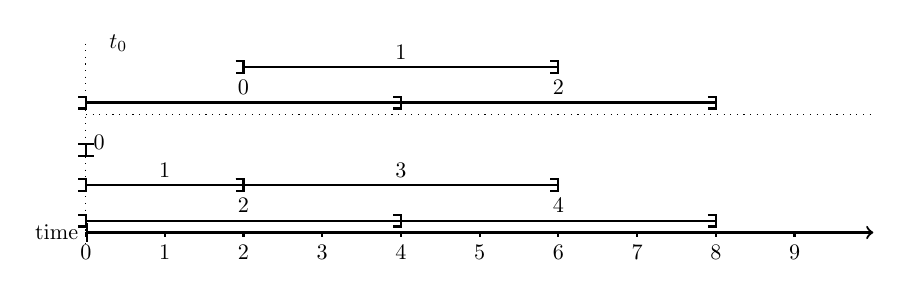
\begin{tikzpicture}[xscale=1, yscale=0.3, every node/.style={scale=0.8}]
\node [left] at (0,0) {time};
\draw [thick,|->] (0,0) -- (10,0);

\seg{0}{0}{3.5}-+\node [right] at (0,3.8){0};
\seglbl{0}{2}{2}--{1};
\seglbl{0}{4}{0.5}--{2};
\seglbl{2}{6}{2}--{3};
\seglbl{4}{8}{0.5}--{4};
\draw [dotted] (0,8) -- (0,-0.5); \node [right] at (0.2,8) {$t_0$};

\seglbl{4}{8}{5.5}--{2};
\seglbl{2}{6}{7}--{1};
\seglbl{0}{4}{5.5}--{0};
\draw [dotted] (0,5) -- (10,5);
\lgrad{0} \lgrad{1} \lgrad{2} \lgrad{3} \lgrad{4} \lgrad{5} \lgrad{6} \lgrad{7} \lgrad{8} \lgrad{9} 
\end{tikzpicture}
\caption{Différence entre les sémantiques avec ou sans $\max$ dans la description RANGE 4 SLIDE 2}\label{fig:valid:expressivite:slidemax}
\end{figure}

Nous pouvons remarquer que nous avons aussi introduit la notion d'inclusion de bornes. Ce qui permet de clarifier si la borne inférieure est incluse dans le contenu de la fenêtre. Dans le cadre des fenêtres glissantes ce n'est pas le cas~\footnote{Il est intéressant de noter un erratum dans la spécification de cet opérateur où la définition précise que la borne inférieure est incluse alors que les exemples et les expérimentations pratiques indiquent le contraire.}.

\subsubsection{RANGE $x$}
Dans ses définitions usuelles, RANGE $x$ seule est possible et est similaire à RANGE $x$ SLIDE 1. Dans Astral, le temps n'est pas discret et une telle définition n'a pas de sens. Une définition similaire est possible en supposant que le \textit{chronon} du système d'implémentation est $\varepsilon$, alors : RANGE $x$ = RANGE $x$ SLIDE $\varepsilon$.

Une approche plus propre serait d'utiliser une DSF générique en basant ses instants d'évaluations (fournis par $\gamma$, pour rappel) sur les arrivés et départs d'n-uplets dans la fenêtre. Toutefois une connaissance de $\alpha^{-1}$ et $\beta^{-1}$ est nécessaire et rend son expression plus complexe. Il est intéressant de voir que ce comportement est telle qu'implémenté car un opérateur vérifiant à chaque \textit{timestamp} système si un n-uplet doit sortir de la fenêtre n'est pas efficace. Il est plus efficace de planifier (via le \textit{scheduler}) ses instants d'évaluations.

\subsubsection{Descriptions à bornes linéaires}
Dans SStreamWare~\cite{Gurgen:sstreamware}, les fenêtres sont définies par un 5-uplet (start, end, rate, start\_adv, end \_adv) :
\begin{itemize}
	\item start (resp. end) décrit la borne inférieure (resp. supérieure) de la première fenêtre produite par la séquence
	\item rate est la fréquence d'évaluation
	\item start\_adv (resp. end\_adv) décrit la quantité de glissement de la borne inférieure (resp. supérieure) à chaque évaluation.
\end{itemize}

Dans Astral, ce comportement est facilement représentable sous forme de DSF :
\DSF{r = \textrm{rate}}
	{\beta(j) = \textrm{end\_adv}*j+\textrm{end}}
	{\alpha(j) = \textrm{start\_adv}*j+\textrm{start}}

\subsubsection{Descriptions procédurales}
Dans les premières versions de TelegraphCQ~\cite{Chandrasekaran:telegraphcq}, les descriptions de fenêtres étaient faites par une boucle \textit{for} procédurale sur un \textit{timestamp} :
\begin{lstlisting}[language=C]
for(t = init ; continue(t) ; t = evolution(t))
	WindowIs(S, begin(t), end(t))
\end{lstlisting}

Ceci peut être formalisé grâce à une DSF générique. Considérons la suite suivante : $u_0=$ init, $u_n=$ evolution($u_{n-1}$) si continue($u_{n-1}$) est vraie, $u_n = u_{n-1}$ sinon. Alors, nous obtenons la description suivante :

\DSF{\gamma(t,i) = \displaystyle\sum_{i=0}^{+\infty} u_i \indic_{[u_i, u_{i+1}[}(t)}
	{\beta = \textrm{end}}
	{\alpha = \textrm{begin}}

La fonction $\gamma$ est définie par une liste de points. Cette définition est courante pour les définitions des fonctions en escaliers. Il est notable que pour des fenêtres avec un taux d'évaluation constant et une position initiale usuelle, une DSF simplifiée est suffisante. 
\subsubsection{Description multi-domaines}
Dans certains systèmes d'observations~\cite{Jurdak:sumac}, il est courant de récupérer les données par vague. Ainsi, dans les interfaces d'observations, nous pouvons régulièrement voir des séquences de fenêtres \enquote{les $n$ derniers n-uples toutes les $m$ secondes}. Pour formaliser une telle séquence, il n'est pas nécessaire d'utiliser une DSF générique car l'évaluation reste périodique. Voici la description de la séquence précédemment décrite :

\DSF{r=m}
	{\beta(j) = \rtau(mj+t_0)}
	{\alpha(j)= \max(\rtau_S(mj+t_0)-n,0)}

Le taux est temporel et les bornes sont positionnelles. Le pont entre les domaines est assuré par l'opérateur grâce aux fonctions $\tau_S$ et $\rtau_S$. Dans ce cas, l'expression $\rtau_S(mi+t_0)$ donne la position à un \textit{timestamp} donné. La remarque concernant le $\max$ que nous avions faite plus tôt reste valable ici.

\subsubsection{Introduction d'un délai}
Dans les travaux de Patroumpas et Sellis~\cite{Patroumpas:window}, l'introduction d'un délai de traitement a été formalisée. En effet, si un n-uplet possède un \textit{timestamp} légèrement déphasé par rapport à son temps réel, alors la fenêtre peut tout de même l'inclure.

Sa formalisation dans notre cas revient à légèrement changer notre fonction $\gamma$ par $\gamma'$ qui décale l'évaluation de $\delta$. Par exemple, nous obtenons pour une description temporelle : $$\gamma'(t,i) = \gamma(t-\delta,i) = \left\lfloor\frac{t-\beta(0)-\delta}{r}\right\rfloor$$

\subsubsection{Modèle d'exécution de SECRET}
Enfin, SECRET~\cite{Botan:secret} est un modèle permettant de généraliser les sémantiques d'exécutions des fenêtres. L'approche est de découper l'exécution d'une fenêtre en quatre concepts que nous pouvons retrouver dans Astral.
\begin{itemize}
	\item Les \textit{Ticks} décident du moment où le système doit réagir au flux (sémantique basé n-uplet, basé temps ou \textit{batch}).
	\item Le \textit{Content} défini le contenu global de la fenêtre par son \textit{Scope}, c'est à dire sa description.
	\item Enfin, un \textit{Report} envoie le résultat final.
\end{itemize}

Bien que les approches soient différentes : nous retrouvons des notions similaires. Le \textit{Scope} est similaire à $\alpha$, $\beta$. Le \textit{Content} à une fenêtre en particulier. Les \textit{Ticks} et les \textit{Reports} sont faites grâce à la fonction $\gamma$ et le contrôle du mode d'exécution par les opérateurs \textit{SPREAD}. L'avantage de l'approche de SECRET est de pouvoir qualifier rapidement le comportement de l'exécution d'un SGFD en particulier, alors qu'Astral décrit la sémantique exacte du résultat pour l'utilisateur.

Nous avons désormais détaillé le positionnement de l'opérateur de séquence de fenêtre par rapport à la littérature. Nous constatons que l'opérateur permet de couvrir l'ensemble des sémantiques actuellement découvertes. Nous avons clarifié plusieurs descriptions non-triviales telles que les fenêtres RANGE stricte, les fenêtres multi-domaines et l'introduction du délai. Nous présentons maintenant l'analyse de l'opérateur de manipulation temporelle.

\subsection{Manipulation temporelle}
L'opérateur de manipulation temporelle (def~\ref{def:manipulation}) permet de transformer le temps \textit{courant} en un temps passé. Ceci permet de transformer le moment d'évaluation de la relation temporelle. Dans l'état actuel de l'art, à notre connaissance, il n'existe pas d'opérateur capable de faire explicitement cette opération. Dans notre cas, il a permit à Asteroid de manipuler facilement la sémantique de mise à jour des relations issues d'un SGBD.

Cet opérateur nous a permit notamment d'introduire la jointure semi-sensible $\ssjoin$. Cette jointure permet de refléter un comportement qui se retrouve dans plusieurs SGFD : ne réagir que sur les mises à jours d'une seule branche.

Une autre application intéressante de cet opérateur est le calcul de changement d'une relation temporelle. Comme nous l'avons vu, l'opérateur $\IS$ est capable de fournir les nouveaux n-uplets d'une relation. Nous pouvons toutefois avoir un résultat pouvant être très intéressant dans le cadre l'observation de système : \enquote{A partir d'une relation temporelle $R$($id$,$v$), fournir le flux des changements ($id$,$v$,$v_{old}$) avec $v_{old}$ l'ancienne valeur pour l'identifiant $id$}. Cette requête s'écrit ainsi :
$$\IS(R \Join_{v\neq v_{old}} (D^{(t,i)^-}_{t>t_0}\rho_{v_{old}/v} R))$$
L'opérateur $D^{(t,i)^-}_{t>t_0}$ retarde la relation temporelle d'un \textit{batch}. Il devient possible d'interroger à un instant donné, une relation temporelle et son état précédent. Les \textit{streamers} permettent de faire cela en faisant une jointure implicite sur $\varphi$. Cette opération est une décomposition permettant de joindre sur tout attribut.

Nous avons présenté l'ensemble des aspects novateurs des définitions d'Astral. Nous détaillons maintenant les manipulations possibles grâce à cette algèbre avec un ensemble de propositions et de théorèmes.
\section{Propositions et théorèmes}
Dans cette section, nous explorons les équivalences de requêtes possibles grâce à Astral. Premièrement, nous explorons comment le \textit{timestamp} et les \textit{batchs} sont conservés malgré l'utilisation de \textit{streamers}, et les conséquences que cela implique. Ensuite, nous explorons les relations classiques de commutativité et d'associativité des opérateurs, ce qui a des impacts nets lors de l'optimisation logique. Enfin, nous présentons les résultats de calculs de transposibilité.

\subsection{Transmission du temps}
La définition~\ref{def:stamping} de la réécriture des n-uplets des \textit{streamers} implique le changement de son \textit{timestamp} et de son \textit{batch}. Ainsi, lors de l'application successive d'un opérateur de séquence de fenêtre et d'un \textit{streamer} : il n'est pas trivial de voir que ces propriétés seront conservés. Le théorème~\ref{thm:transmission} de transmission temporelle permet d'avoir une condition suffisante pour garantir cette transmission.

\begin{thm}[Transmission temporelle des \textit{streamers}]\label{thm:transmission}
    Soit $S$ un flux,

    Soit $]\!\![\alpha,j+k,1]$ une DSF positionnelle avec $\alpha$ croissante et $k$ un entier, 

    Considérant $S'$ le flux formé par la requête $\IS(S]\!\![\alpha,i+k,1])$,

    Si un n-uplet réécrit de $S'$ a pour \textit{batch} $(t,i)$ alors, ce n-uplet avait originellement pour \textit{batch} $(t,i)$ dans $S$. Formellement :
$$\Psi_{(t,i)}(s,t) \wedge \B{S'}(\Psi_{(t,i)}(s,t)) = (t,i) \im s\in S \wedge \BS(s) = (t,i)$$

    Cette propriété est aussi valable pour $\RSu(S[B])$.
\end{thm}

Le corrolaire à ce théorème est le fait que $\IS$ peut être vu comme l'opération inverse d'une fenêtre $[B]$ par exemple.
\begin{coro}[Équivalence de la composition fenêtre-\textit{streamer}]
    Sachant une composition de fenêtre-streamers respectant les conditions du théorème~\ref{thm:transmission},

    Si $\alpha$ est telle que la séquence de fenêtre contient $[B]$, alors,
$$S \equiv \IS(S]\!\![\alpha,i+k,1n]) \equiv \IS(S[B]) \equiv \IS(S[\infty]) \equiv \RSu(S[B])$$
\end{coro}

\begin{example}
Reprenons l'exemple vu dans la section~\ref{sec:contrib:astral:definitions:exemple} avec le flux \textbf{CPU}(appId, cpu, $\t$). En prenant la fenêtre $[B]$, le corollaire nous assure que $\IS(S[B])=S$. L'insertion d'un n-uplet dans le flux est effectuée à un \textit{batch} égal au \textit{batch} du n-uplet initial. Ainsi, l'opérateur $\IS$ écrasera le \textit{timestamp} avec celui du \textit{batch}. Voici la suite des états par lesquels passe la relation temporelle $CPU[B]$, ainsi que le flux résultant de $\IS(CPU[B])$ :
$$CPU(\textrm{id},\textrm{cpu},\t)=\{(1,v1,3);(2,v2,9);(1,v3,10);(3,v4,12);...\}$$
\noindent\begin{minipage}[c]{0.24\linewidth}
\begin{center}$CPU[B](3)$: \\ \vspace{1em}
\begin{tabular}{|c|c|c|}
\hline
id & cpu & $\t$ \\
\hline
$1$ & $v1$ & $3$ \\
\hline
\end{tabular}\end{center}
\end{minipage} % Ne pas sauter de ligne !
\begin{minipage}[c]{0.24\linewidth}
\begin{center}$CPU[B](9)$: \\ \vspace{1em}
\begin{tabular}{|c|c|c|}
\hline
id & cpu & $\t$ \\
\hline
$2$ & $v2$ & $9$ \\
\hline
\end{tabular}\end{center}
\end{minipage} % Ne pas sauter de ligne !
\begin{minipage}[c]{0.24\linewidth}
\begin{center}$CPU[B](10)$: \\ \vspace{1em}
\begin{tabular}{|c|c|c|}
\hline
id & cpu & $\t$ \\
\hline
$1$ & $v3$ & $10$ \\
\hline
\end{tabular}\end{center}
\end{minipage} % Ne pas sauter de ligne !
\begin{minipage}[c]{0.24\linewidth}
\begin{center}$\IS(CPU[B])$: \\
\begin{tabular}{|c|c|c|}
\hline
id & cpu & $\t$ \\ \hline
$1$ & $v1$ & $3$ \\ \hline
$2$ & $v2$ & $9$ \\ \hline
$1$ & $v3$ & $10$ \\ \hline
... & ... & ... \\ \hline
\end{tabular}\end{center}
\end{minipage} % Ne pas sauter de ligne !

Nous avons vu que la propriété était effectivement vraie. Voyons maintenant un contre-exemple avec une fenêtre ne respectant pas les conditions du théorème. Nous considérons maintenant l'utilisation de la fenêtre temporelle glissante de $2$ secondes : $[T\ 2s\ 2s]=[W]$. Comme la production d'un n-uplet dans un \textit{streamer} sensible est dirigée par les changements de fenêtres, alors le \textit{timestamp} des n-uplets produits est le moment où le contenu de la fenêtre change. Dans le cas d'une fenêtre changeant toutes les $2$ secondes, cela ne correspond pas au \textit{timestamp} original.

Voici la suite des états par lesquels passe la relation temporelle $CPU[W]$, ainsi que le flux résultant de $\IS(CPU[W])$ :

\noindent\begin{minipage}[c]{0.24\linewidth}
\begin{center}$CPU[W](4)$: \\ \vspace{1em}
\begin{tabular}{|c|c|c|c|}
\hline
id & cpu & $\t$ \\
\hline
$1$ & $v1$ & $3$ \\
\hline
\end{tabular}\end{center}
\end{minipage}  % Ne pas sauter de ligne !
\begin{minipage}[c]{0.24\linewidth}
\begin{center}$CPU[W](10)$: \\ \vspace{1em}
\begin{tabular}{|c|c|c|c|}
\hline
id & cpu & $\t$ \\
\hline
$2$ & $v2$ & $9$ \\ \hline
$1$ & $v3$ & $10$ \\ \hline
\end{tabular}\end{center}
\end{minipage} % Ne pas sauter de ligne !
\begin{minipage}[c]{0.24\linewidth}
\begin{center}$CPU[W](12)$: \\ \vspace{1em}
\begin{tabular}{|c|c|c|c|}
\hline
id & cpu & $\t$ \\
\hline
$3$ & $v4$ & $12$ \\ \hline
\end{tabular}\end{center}
\end{minipage} % Ne pas sauter de ligne !
\begin{minipage}[c]{0.24\linewidth}
\begin{center}$\IS(CPU[W])$: \\ \vspace{1em}
\begin{tabular}{|c|c|c|c|} \hline
id & cpu & $\t$ \\ \hline
$1$ & $v1$ & $4$ \\ \hline
$2$ & $v2$ & $10$ \\ \hline
$1$ & $v3$ & $10$ \\ \hline
$3$ & $v4$ & $12$ \\ \hline
... & ... & ... \\ \hline
\end{tabular}\end{center}
\end{minipage}

Ainsi, nous avons bel et bien la relation suivante : $I_S(CPU[T\ 2s\ 2s]) \not\equiv CPU$.
\end{example}

Ce résultat permet de traiter des flux d'une manière pratique. Un flux $S$ n'est pas manipulable a priori par une implémentation car c'est une entité infinie. Par contre, $S[B]$ correspond au \textit{dernier batch} qui est accessible. Ainsi, la lecture d'un flux correspond à la récupération du dernier \textit{batch} et envoyer les n-uplets dans le flux résultant. De plus, lorsque le dernier \textit{batch} est récupéré, il est possible d'y appliquer des opérations simples avant de le renvoyer. Nous définissons les sélections, projections et renommage sur flux par l'application de ces opérations sur la fenêtre \textit{batch}.

\begin{coro}[Définition de la sélection, projection et renommage sur flux]
    Soit $S$ un flux,

    Soit $\nu$ un opérateur pouvant être $\sigma$, $\Pi$ ou $\rho$,

    Son application sur un flux est définie par :
$$\nu S = \IS(\nu(S[B]))$$
\end{coro}

Afin de montrer que cette définition est viable, nous facilement démontrer grâce au théorème~\ref{thm:transmission} que la sélection sur flux correspond à la sémantique intuitive. $$\sigma_c(S) = \IS(\nu(S[B])) = \{s\in S, c(s)\}$$

\subsection{Commutativité et associativité}
Nous voyons désormais les règles de commutativité et d'associativité. Ces règles étaient déjà existantes dans le cadre de l'algèbre relationnelle. Nous les redécouvrons ici. Nous détaillons premièrement les projections.

L'opérateur de projection a peu d'impact dans la sémantique des opérateurs. Les règles sont principalement issues de l'algèbre relationnelle qui nous donne beaucoup de résultats. Comme la projection ne perturbe pas les cardinalités ou les ordres, il n'y a pas d'impact non désirés. De plus, l'opérateur permute facilement avec la fenêtre et les \textit{streamers}. Le tableau~\ref{tab:projection} référence l'ensemble des règles de transformations pour pousser les projections au plus proche des sources.

\begin{table}[p]
\centering
($E$ = entité, $R$ = relation temporelle, $S$ = flux)
\begin{tabular}{|c|c|c|} \bottomrule
\rowcolor{hypcolor} Hypothèse & Condition & Résultat \\ \hline
    $\Pi_a E$ & $a = attr(E)$ & $E$ \\ \hline
    $\Pi_a \Pi_b E$ & & $\Pi_a E$ \\ \hline
    $\Pi_a \sigma_c E$ & &  $\Pi_{a}\sigma_c \Pi_{a\cup attr(c)} E$  \\ \hline
    $\Pi_a e_{f(b)}^c E$ & &  $\Pi_{a} e_{f(b)}^c \Pi_{(a \backslash c)\cup b} E$  \\ \hline
    \multirow{2}{*}{$\Pi_{a} \rho_{y/x} E$} & $y \in a$ & $\rho_{y/x}\Pi_{a\backslash\{y\},x}  E$ \\ \cline{2-3}
    & $y \not\in a$ & $\rho_{y/x}\Pi_{a} E$ \\ \hline
    $\Pi_{a}(R_1\Join R_2)$ & &  $\Pi_{a}(\Pi_{Attr(R_1)\cap a} R_1\Join \Pi_{Attr(R_2)\cap a} R_2)$  \\ \hline
    $\Pi_{a} S[\alpha,\beta,\gamma]$ & &  $(\Pi_{a\cup \t} S)[\alpha,\beta,\gamma]$  \\ \hline
    $\Pi_{a} \IS(R)$ &  & $\IS(\Pi_{a\backslash \t} R)$ \\ \hline
    $\Pi_{a} \DS(R)$ &  & $\DS(\Pi_{a\backslash \t} R)$ \\ \hline
    $\Pi_{a} \RSu(R)$ &  & $\RSu(\Pi_{a\backslash \t} R)$ \\ \hline
    $\Pi_{a} \RS{r}(R)$ & & $\RS{r}(\Pi_{a\backslash \t} R)$ \\ \hline
    $\Pi_{a} \D_c^f(R)$ & & $\D_c^f(\Pi_{a} R)$ \\ \hline
    $\Pi_{a} \ {}_{b} G_{f(c)} R$ & & $\Pi_{a}\  {}_{b} G_{f(c)}  \Pi_{b \cup c} R$ \\ \hline
    $\Pi_{a} (R_1\cup R_2)$ & &  $(\Pi_{a} R_1)\cup (\Pi_{a} R_2)$  \\ \toprule
\end{tabular}
\caption{Table des règles de commutativité de la projection $\Pi$}\label{tab:projection}
\end{table}
\begin{table}[p]
\centering
($E$ = entité, $R$ = relation temporelle, $S$ = flux)
\begin{tabular}{|c|c|c|} \bottomrule
\rowcolor{hypcolor} Hypothèse & Condition & Résultat \\ \hline
    $\sigma_c \sigma_{c'} E$ & & $\sigma_{c\wedge c'} E$ \\ \hline
    $\sigma_c e_{f(b)}^a E$ & $a \not\in attr(c)$ & $e_{f(b)}^a \sigma_c E$ \\ \hline
    \multirow{2}{*}{$\sigma_c \rho_{y/x} E$} & $x \in attr(c)$ & $\rho_{y/x}\sigma_{\textrm{replace}(x,y,c)}  E$ \\ \cline{2-3}
    & $x\not\in attr(c)$ & $\rho_{y/x}\sigma_c E$ \\ \hline
    \multirow{3}{*}{$\sigma_c(R_1\Join_d R_2)$} & $attr(c)\subseteq attr(R_1)\backslash attr(R_2)$ & $(\sigma_c(R_1)) \Join_d R_2$  \\ \cline{2-3}
    & $attr(c)\subseteq attr(R_2)\backslash attr(R_1)$ & $R_1 \Join_d (\sigma_c(R_2))$ \\ \cline{2-3}
    & sinon & $R_1 \Join_{d \wedge c} R_2$  \\ \hline
    \multirow{2}{*}{$\sigma_c S[\alpha,\beta,\gamma]$} & $[\alpha,\beta,\gamma]=[\infty]$ & \multirow{2}{*}{$(\sigma_c S)[\alpha,\beta,\gamma]$} \\ \cline{2-2}
     & $\alpha,\beta,\gamma$ temporels & \\ \hline
    $\sigma_c \IS(R)$ &  & $\IS(\sigma_c R)$ \\ \hline
    $\sigma_c \DS(R)$ &  & $\DS(\sigma_c R)$ \\ \hline
    $\sigma_c \RS{r}(R)$ & & $\RS{r}(\sigma_c R)$ \\ \hline
    $\sigma_c \D_c^f(R)$ & & $\D_c^f(\sigma_c R)$ \\ \hline
    $\sigma_c \ {}_{b} G_{f(c)} R$ & $attr(c)\subseteq b$ & $\sigma_c\  {}_{b} G_{f(c)}  \Pi_{b \cup c} R$ \\ \hline
    $\sigma_c (R_1\cup R_2)$ & &  $(\sigma_c R_1)\cup (\sigma_c R_2)$  \\ \toprule
\end{tabular}
\caption{Table des règles de commutativité de la sélection $\sigma$}\label{tab:selection}
\end{table}


La sélection est quant à elle plus délicate. En effet, elle perturbe la cardinalité du flux. Ainsi, l'opérateur de fenêtre dans le cas positionnel peut ne pas sélectionner les mêmes n-uplets. Il est possible de fournir un contre-exemple interdisant la permutation avec l'opérateur de fenêtre.
\begin{example}
Soit le flux exemple $CPU$, considérons les requêtes suivantes :
\begin{enumerate}
	\item $\sigma_{cpu>50} (CPU[N\ 10\ 1])$ est l'ensemble des relevés supérieurs à 50\% des 10 dernières mesures à chaque nouvelle mesure.
	\item $(\sigma_{cpu>50} CPU)[N\ 10\ 1])$ est l'ensemble des 10 dernières valeurs des relevés supérieurs à 50\% chaque nouvelle mesure >50\%.
\end{enumerate}
Les tailles des fenêtres de ces requêtes sont différentes. Dans la seconde requête, la largeur est constante à 10 n-uplets. Alors que dans le premier cas, s'il existe des n-uplets $\leq 50\%$ alors la taille sera $<10$ n-uplets.
\end{example}
Le problème dépend du fait que $\tau_{\sigma_c S}$ et $\tau_S$ sont deux fonctions différentes. Ce qui impliquera des changements importants dans le cadre de l'opérateur de fenêtre positionnel. Toutefois, dans le cadre particulier des fenêtres temporelles ainsi que de la fenêtre accumulative $[\infty]$ la commutativité est juste\footnote{Car ces définitions de fenêtres ne dépendent pas de la fonction $\tau_S$}. De façon similaire, la commutativité avec $\RSu$ n'est pas autorisé. Les autres règles autorisant la commutativité sont pour la plupart issues de l'algèbre relationnel. La table~\ref{tab:selection} liste l'ensemble des règles pour pousser les sélections.

Nous abordons maintenant la question de l'associativité. Dans le cadre de nos définitions par défaut, les associativités issues de l'algèbre relationnelles sont toujours vraies.
\begin{thm}[Associativité des jointures et unions]
Les opérations de jointure et d'union sont associatives pour les définitions par défaut de $\Phi^\times$ et $\Phi^\cup$.
\end{thm}
Ceci est dû au fait que l'ordre lexicographique est lui aussi un ordre associatif. En effet, les ordres lexicographiques induits par $\I\times(\I\times\I)$ ou $(\I\times\I)\times \I$ sont équivalents (démonstration simple). Si une autre fonction est utilisée (par exemple, un des jointures est dans l'ordre lexicographique inversé), il est nécessaire de vérifier que les ordres fournis sont toujours équivalents.

Enfin, une dernière commutativité est notable : la manipulation temporelle. Sa commutativité est intuitive à appréhender.
\begin{thm}
L'opérateur de manipulation temporelle est commutatif avec tous les opérateurs relationnels.
\end{thm}
En effet, la manipulation temporelle applique une fonction $f$ au \textit{batch} utilisé pour récupérer la relation instantanée d'une relation temporelle. Or, les opérateurs relationnels sont décomposables comme $\nu (R)(b) = \nu' R(b)$. L'application d'une fonction $f$ donne : $\nu (R)(f(b)) = \nu' R(f(b))$, et $R(f(b))$ correspond à l'application de la manipulation temporelle.

Nous avons donc vu plusieurs propriétés utilisables par les implémentations et optimiseurs. Nous avons désormais plusieurs outils pour appliquer une optimisation logique suffisamment efficace. Nous explorons désormais la transposabilité, qui peut avoir un impact dans le cadre des partages de requêtes.

\subsection{Transposabilité}
Transposabilités simples

Théorème général des fenêtres

Application au cas linéaire

\section{Conclusion}
Ce chapitre a dressé un état de l'art des différents systèmes capables d'offrir une solution générique de supervision. Il en ressort qu'aucun système ne supporte entièrement les critères de qualité que nous nous sommes fixés. Le tableau~\ref{tab:rw:supervision:bilan} résume les 11 points d'analyse en colorant les différentes points suivant leurs conformités. 

\begin{sidewaystable}[ht]
\centering
\begin{tabular}{@{{\vrule width 1pt}\ \ }>{\raggedleft}m{3cm}@{\ \ {\vrule width 1pt}\ \ }M{4.2cm}|M{4.2cm}|M{4.2cm}|M{4.2cm}@{\ \ {\vrule width 1pt}}} \bottomrule
\head Critère & \head Système d'administration & \head Gestion de contexte & \head Entrepôts de données & \head Gestion de flux de données \\  \toprule \bottomrule
\critereAA & Hiérarchique & Triplets & Relationnel & Relationnel dérivé \\ \hline
\critereAB & \meh Structure hiérarchique sans contraintes & \good Ontologies & \good Modèle relationnel normalisé & \bad Pas de structure \\ \hline
\critereAC & \meh Notifications & \bad Ajout du temps en propriété & \meh CDC & \good Flux natif \\ \toprule \bottomrule
\critereBA & \meh Instantanée, continu en ad-hoc & \bad Instantané principalement & \meh Instantané. ETL en pseudo-continu & \bad Continu uniquement \\ \hline
\critereBB & \good Standardisation, union de modèles & \meh Fusion d'ontologies non standardes & \good Processus ETL (complexe) & \good Union et jointures de flux \\ \hline
\critereBC & \bad Impératif principalement & \good Logique & \meh Déclaratif (SQL) et Procédural (ETL) & \good Déclaratif principalement\\ \hline
\critereBD & \meh Procédures à écrire soi-même & \good Logique du premier ordre & \good Relationnel multidimensionnel et Algorithmie dédiée & \meh Relationnel avec support du dynamisme\\ \toprule \bottomrule
\critereCA & \good Support des standards & \meh Spécification longue des domaines & \bad Spécification du schéma, des ETL, autre (complexe) & \good Écriture de requêtes \\ \hline
\critereCB & \bad Aucune & \good Séparation par les domaines & \good Données multidimensionnelles & \bad Aucune \\ \hline
\critereCC & \good Modèle extensible, fonctions métiers dans le gestionnaire & \meh Capteurs virtuels & \good Opérateurs ETL, procédures SQL, algorithmes & \meh Sources et puits mais pas les opérateurs  \\ \hline
\critereCD & \good Large échelle & \bad Complexité très haute & \meh Réactivité lente, Support de grande quantité & \good Support de haut débits\\ \toprule 
\end{tabular}
\caption{Récapitulatif de l'état de l'art des systèmes génériques de supervision}\label{tab:rw:supervision:bilan}
\end{sidewaystable}
Il en ressort que les systèmes d'administrations sont avant tout des systèmes qui fonctionnent grâce au support des standards et à leur simplicité d'implémentation. L'architecture avec gestionnaire adaptable grâce à des langages impératifs permets une grande flexibilité pour s'adapter aux cas d'usages. De son côté, l'informatique contextuelle fournit des outils permettant de modéliser et manipuler proprement les concepts du système grâce aux ontologies et aux raisonnements logiques. Il en sort une claire séparation des domaines de compétences. Les entrepôts de données quant à eux se distinguent par des capacités d'analyses très poussées, ainsi qu'un procédé d'intégration, très complexe et lourd malheureusement, mais très complet. Enfin, la gestion de flux de données est une base solide pour gérer les données dynamiques. L'intégration et l'adaptation au système étant fait entièrement de manière déclarative en fait une solution performante et viable.

À la vue de l'état de l'art, voici les points qui vont être critique sur notre établissement de notre contribution :
\begin{itemize}
    \item La gestion de flux est un bon socle pour gérer les données dynamique grâce aux requêtes continues.
    \item Elle ne suffit pas pour constituer un système d'observation complet, notamment à l'absence de modèle de description et de requêtes instantanées.
    \item Les entrepôts et bases de données sont capables de répondre aux requêtes instantanées.
    \item Les ETL sont trop complexes à manipuler pour intégrer les données, alors que les SGFD sont plus déclaratifs.
\end{itemize}
Il devient clair que les systèmes de gestions de flux de données forment un bon candidat comme fondation pour un architecture d'observation de système. Il nous faut donc approfondir l'état de l'art technique sur ce domaine pour modeler notre contribution. Le point majeur sera d'apporter les capacités des systèmes de gestions de données relationnels. En effet, en apportant le support persistant à la gestion de flux de données, en clarifiant et augmentant son langage, nous aurons un outil qui sera plus apte à répondre à notre problématique. Ainsi, l'héritage du relationnel permettra une structure sémantique correcte, ainsi que des capacités d'analyses plus évoluées. Enfin et surtout, les données serait intégrés malgré leur hétérogénéité profonde. Le chapitre suivant détaille l'état de l'art technique de la gestion de flux de données afin de pouvoir effectuer ces améliorations.
